\documentclass[main.tex]{subfiles}
\begin{document}
\glsresetall

\section{Introduction}

A \gls{rf} is a supervised learning algorithm that uses an ensemble of several decision trees \cite{breiman2001random}.
Decision trees are flow-chart-like structures where each internal node denotes a test on a selected feature. The result is a split in the dataset depending on the value of that feature. The best splitting criterion for regression is typically calculated using the \gls{mse}. For each node, the \gls{mse} of the two subsets is calculated for each feature and for each possible cut on that feature, until a minimum is reached. This step is repeated at each node until a condition is reached, typically that the \gls{mse} of the remaining data sample is below a threshold, or it has too few events to keep splitting. The termination nodes are also known as \textit{leaves}. For classification, the splitting criterion is based on the gini index, described in section \ref{sec:giniidx}.
In the \gls{rf}, several decision trees are trained using a randomly selected subset of the train data (\textit{'bootstrapping'}) and the prediction of all the trees is averaged to reach the final result. Also, the features are always randomly permuted at each split. These two sources of randomness in the \gls{rf} prevent the typical problem of over-fitting from too complicated decision trees.

\section{Gini Index} \label{sec:giniidx}

The gini index o gini impurity is a measure of how often a randomly chosen event would be incorrectly classified if it was classified randomly following the distribution of classes. The formula for the Gini index $I_G$ calculated for a set of events with J classes is:

\begin{equation}
  I_G(p) = 1 - \sum_{i=1}^J p_i^2
\end{equation}

Where $p_i$ is the probability of an event belonging to the class $i$ to be correctly classified.  The Gini index goes from 0 to 1, where 0 means that all the events of a subset have been classified into one class, and 1 that the events of the subset are randomly distributed along with all the possible classes. The splitting decision will be made minimizing the value of the Gini index.

\section{Random Forests in cta-lstchain}

\subsection{Random Forest parameters}
The \glspl{rf} applied in this thesis for the analysis performed in chapter \ref{cap:LST} were implemented using the python package \textit{scikit-learn} \cite{2011scikit-learn}. Several configurable parameters can be tuned to improve the performance of the \glspl{rf}. The parameters used in this thesis are summarized in table \ref{tab:RFpars}.

\begin{table}[h!]
  \centering
  \begin{tabular}{|l|l|l|l|}
    \hline
    Parameter name & Value          & Value              & Description\\
    & for regression & for classification &  \\
    \hline
    n\_estimators       & 150 & 100  & \small{Number of trees in the forest}\\
    criterion           & mse & gini & \small{Function to measure the quality of a split}\\
    max\_depth          & 50  & 100  & \small{Maximum depth of the tree}\\
    min\_samples\_split & 2   & 2    & \small{Minimum number of samples required to}\\
    &     &      & \small{split an internal node} \\
    min\_samples\_leaf  & 2   & 2    & \small{Minimum number of samples to be at a}\\
    &     &      & \small{leaf node} \\
    max\_features       & all & all  & \small{Number of features to consider when looking} \\
    &     &      & \small{for the best split}\\
    random\_state       & 42  & 42   & \small{Control the randomness of the} \\
    &     &      & \small{bootstrapping and the sampling of features}\\
    n\_jobs             & 4   & 4    & \small{Number of jobs to run in parallel}\\
    \hline
  \end{tabular}
  \caption{Some parameters that can be configured for \textit{RandomForestRegressor} and \textit{RandomForestClassifier} classes, with the values used in \textit{cta-lstchain} for the training of the \glspl{rf} used in this thesis.}
  \label{tab:RFpars}
\end{table}

\subsection{Random Forest feature importances}

The \gls{rf} assigns an importance score to the different features used for training, where the most relevant have a higher score. Picture \ref{fig:importances} show the importance of the features used to train the \gls{rf} applied to \gls{mc} data to compute the performance of the \gls{lst} in section \ref{sec:performance}.

\begin{figure}[h]
  \centering
  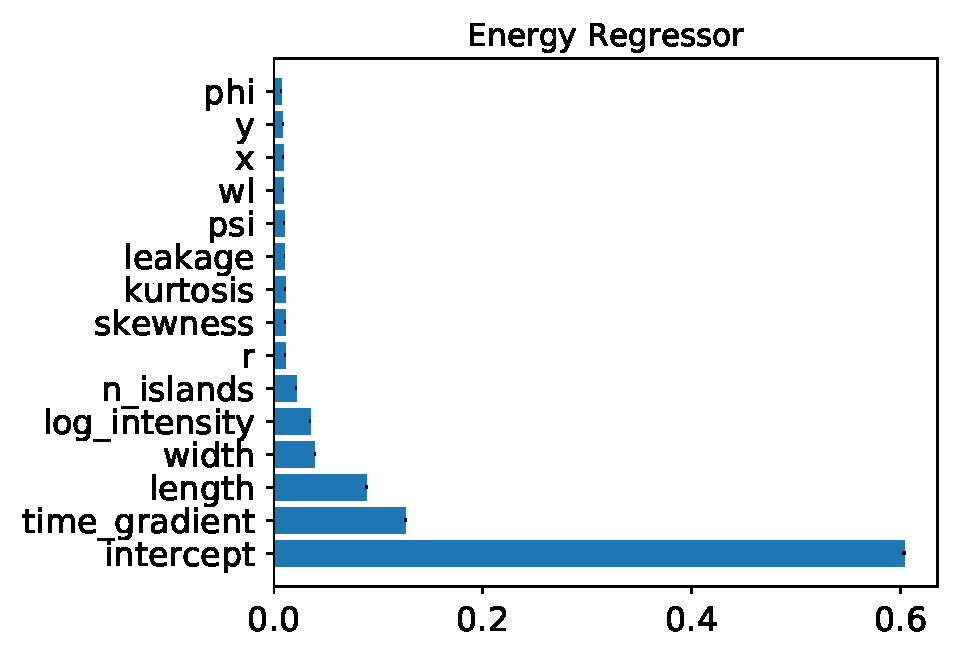
\includegraphics[width=0.45\textwidth]{Pictures/reg_energy_importances.pdf}
  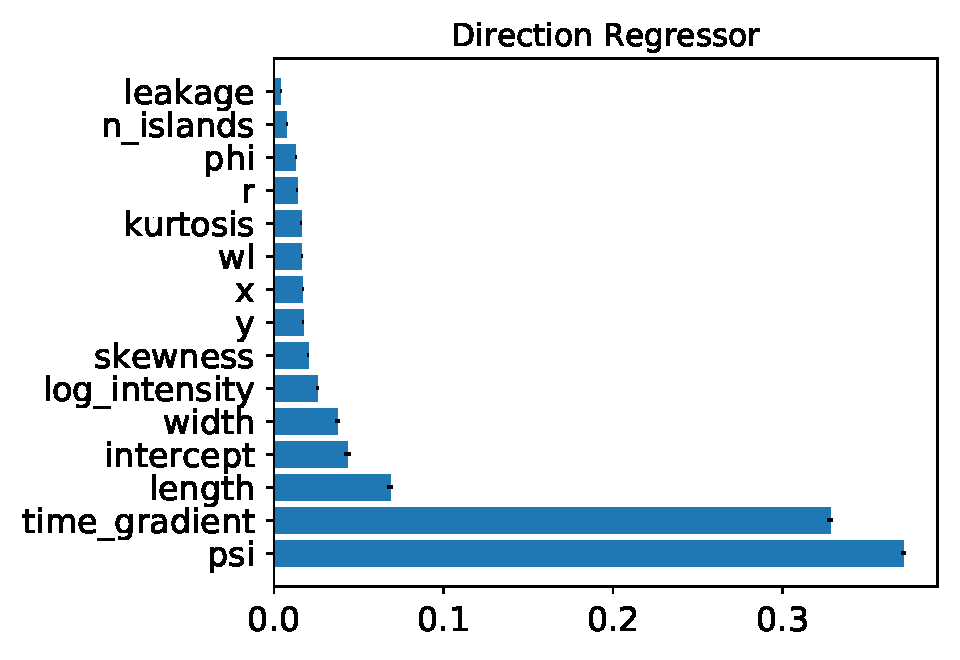
\includegraphics[width=0.45\textwidth]{Pictures/reg_disp_vector_importances.pdf}
  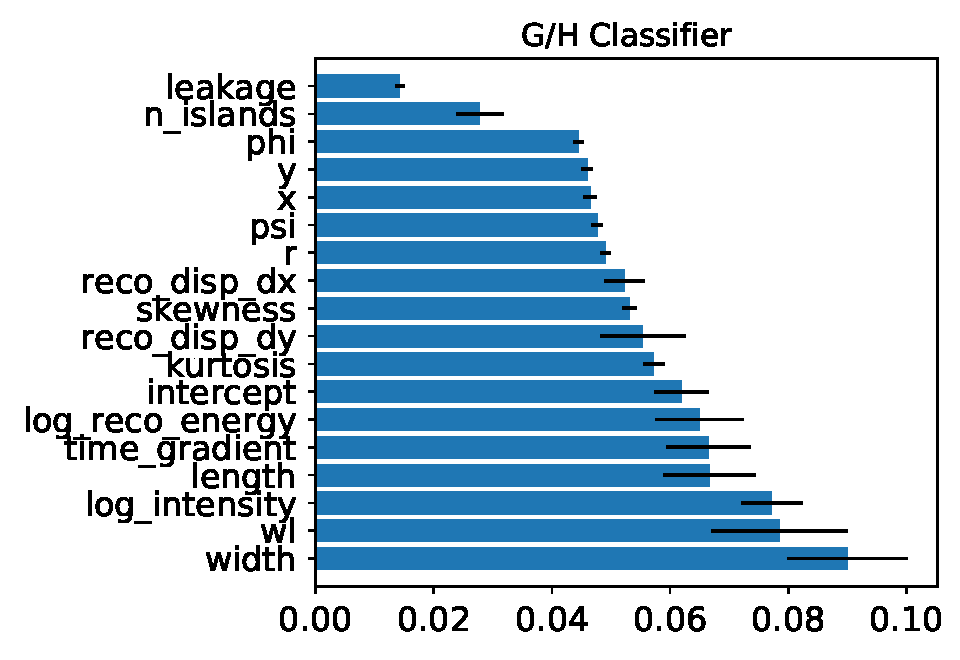
\includegraphics[width=0.45\textwidth]{Pictures/gls_importances.pdf}
  \caption{Parameters importance for the trained \gls{rf} used in the analysis of \gls{mc} simulated \gls{lst}1 data. The higher the importance value, the more relevant is the feature for the regression/classification.}
  \label{fig:importances}
\end{figure}

\end{document}
